\documentclass[12pt]{article}[a4paper,14pt,russian]

 \usepackage{graphicx}
\usepackage[russian]{babel}
\usepackage[utf8]{inputenc}
\usepackage{color}
\usepackage{indentfirst}
\usepackage[margin=2cm]{geometry}
\usepackage{setspace}
\singlespacing
\definecolor{lgreen}{rgb}{0.9,1,0.8}
\definecolor{light-blue}{rgb}{0.8,0.85,1}
\newcommand{\alarm}[1]{\textbf{ПМ "#1"}}
\renewcommand{\figurename}{Рисунок}
\begin{document}
\section{Назначение программы}
Программа <<Коммутатор портов>> предназначена для отображения обмена данными между двумя устройствами, работающими через COM порт. Устройства подключаются к персональному компьютеру на котором запускается программа <<Коммутатор портов>>. Данные, приходящие на <<Порт 1>> от первого устройства автоматически перенаправляются на <<Порт 2>>, подключенный к второму устройству и наоборот. Программа позволяет просматривать протокол обмена между устройствами в формате ASCII либо в шестнадцатеричных кодах.
\section {Выполнение программы}
Для выполнения программы необходимо наличие персонального компьютера под управление операционной системы <<Windows 7>> и выше и как минимум двух устройств, работающих через COM порт.
\subsection{Установка программы}
Для установки программы необходимо запустить инсталлятор
Switch\_com-Win32-0.1.exe. В процессе инсталляции будет предложено выбрать папку для установки программы. Инсталлятор автоматически создаст ярлык на рабочем столе.
\subsection {Запуск программы}
 Для запуска программы нажмите два раза левой кнопкой мыши на ярлыке программы, расположенном на рабочем столе или перейдите в ту папку куда вы установили программу и запустите ее нажав два раза левой кнопкой мыши на файле <<switch.exe>> Перед вами откроется главное окно программы, представленное на рис. ~\ref{ris:image}
 \begin{figure}[h!]
 	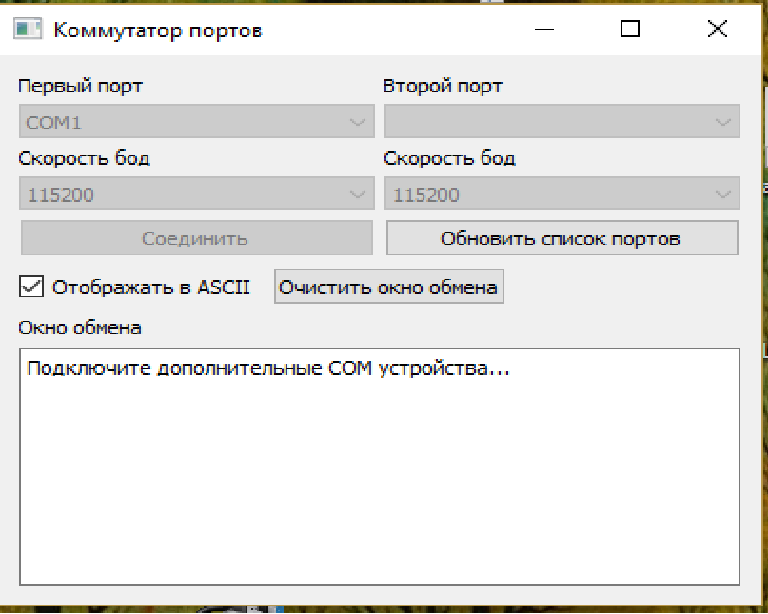
\includegraphics [scale=0.6]{MainWindow.png}
 	\caption{Главное окно программы}
 	\label{ris:image}
 \end{figure}
\section{Работа с программой}
Если в системе присутствует меньше двух COM портов то кнопка "Соединить" будет заблокирована, данная ситуация представленна на рисунке ~\ref{ris:image}. После подключения необходимого количества COM портов необходимо нажать кнопку "Обновить список портов". Программа обнаружит устройства и выведет их в главном окне (рис. ~\ref{ris:connected} ). Для просмотра обмена между устройствами необходимо нажать кнопку "Соединить". Протокол обмена данными между устройствами представлен в окне обмена. Для очистки окна отображения протокола необходимо нажать кнопку "Очистить". Программа позволяет отображать протокол как в шестнадцатеричном видет так и в формате ASCII, для переключения режимов используйте флажок с надписью <<в ASCII>>.
\begin{figure}
	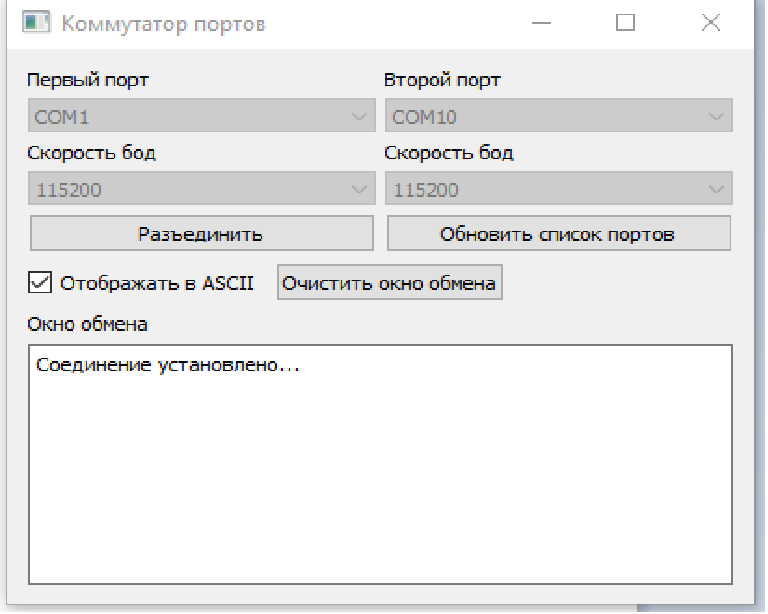
\includegraphics [scale=0.8]{Connected.png}
	\caption{Главное окно программы}
	\label{ris:connected}
\end{figure}
\subsection{Сообщения оператору}
Сообщения оператору отображаются в окне обмена. Перечислим их:
\begin{itemize}
\item <<Подключите дополнительные COM устройства>> - сообщение говорит о том, что система не обнаружила необходимого количества 
COM портов. Необходимо подключить дополнительные устройства и нажать кнопку <<Обновить список портов>>
\item  <<Соединение установлено...>> - сообщение появляется после успешной коммутации портов и обозначает, что программа работает в штатном режиме.
\end{itemize}
\end{document}